\PassOptionsToPackage{unicode=true}{hyperref} % options for packages loaded elsewhere
\PassOptionsToPackage{hyphens}{url}
\documentclass[14pt,ignorenonframetext,compress]{beamer}
\IfFileExists{pgfpages.sty}{\usepackage{pgfpages}}{}
\setbeamertemplate{caption}[numbered]
\setbeamertemplate{caption label separator}{: }
\setbeamercolor{caption name}{fg=normal text.fg}
\beamertemplatenavigationsymbolsempty
\usepackage{lmodern}
\usepackage{amssymb,amsmath}
\usepackage{ifxetex,ifluatex}
\usepackage{fixltx2e} % provides \textsubscript
\ifnum 0\ifxetex 1\fi\ifluatex 1\fi=0 % if pdftex
  \usepackage[T1]{fontenc}
  \usepackage[utf8]{inputenc}
\else % if luatex or xelatex
  \ifxetex
    \usepackage{mathspec}
  \else
    \usepackage{fontspec}
\fi
\defaultfontfeatures{Ligatures=TeX,Scale=MatchLowercase}







\fi

  \usetheme[]{monash}

  \usecolortheme{monashwhite}


% A default size of 24 is set in beamerthememonash.sty




% use upquote if available, for straight quotes in verbatim environments
\IfFileExists{upquote.sty}{\usepackage{upquote}}{}
% use microtype if available
\IfFileExists{microtype.sty}{%
  \usepackage{microtype}
  \UseMicrotypeSet[protrusion]{basicmath} % disable protrusion for tt fonts
}{}


\newif\ifbibliography


\hypersetup{
      pdftitle={Artificial Bee Colony (ABC) algorithm and Clustering},
        pdfauthor={Yangzhuoran (Fin) Yang},
          pdfborder={0 0 0},
    breaklinks=true}
%\urlstyle{same}  % Use monospace font for urls




  \usepackage{color}
  \usepackage{fancyvrb}
  \newcommand{\VerbBar}{|}
  \newcommand{\VERB}{\Verb[commandchars=\\\{\}]}
  \DefineVerbatimEnvironment{Highlighting}{Verbatim}{commandchars=\\\{\}}
  % Add ',fontsize=\small' for more characters per line
  \usepackage{framed}
  \definecolor{shadecolor}{RGB}{248,248,248}
  \newenvironment{Shaded}{\begin{snugshade}}{\end{snugshade}}
  \newcommand{\AlertTok}[1]{\textcolor[rgb]{0.94,0.16,0.16}{#1}}
  \newcommand{\AnnotationTok}[1]{\textcolor[rgb]{0.56,0.35,0.01}{\textbf{\textit{#1}}}}
  \newcommand{\AttributeTok}[1]{\textcolor[rgb]{0.77,0.63,0.00}{#1}}
  \newcommand{\BaseNTok}[1]{\textcolor[rgb]{0.00,0.00,0.81}{#1}}
  \newcommand{\BuiltInTok}[1]{#1}
  \newcommand{\CharTok}[1]{\textcolor[rgb]{0.31,0.60,0.02}{#1}}
  \newcommand{\CommentTok}[1]{\textcolor[rgb]{0.56,0.35,0.01}{\textit{#1}}}
  \newcommand{\CommentVarTok}[1]{\textcolor[rgb]{0.56,0.35,0.01}{\textbf{\textit{#1}}}}
  \newcommand{\ConstantTok}[1]{\textcolor[rgb]{0.00,0.00,0.00}{#1}}
  \newcommand{\ControlFlowTok}[1]{\textcolor[rgb]{0.13,0.29,0.53}{\textbf{#1}}}
  \newcommand{\DataTypeTok}[1]{\textcolor[rgb]{0.13,0.29,0.53}{#1}}
  \newcommand{\DecValTok}[1]{\textcolor[rgb]{0.00,0.00,0.81}{#1}}
  \newcommand{\DocumentationTok}[1]{\textcolor[rgb]{0.56,0.35,0.01}{\textbf{\textit{#1}}}}
  \newcommand{\ErrorTok}[1]{\textcolor[rgb]{0.64,0.00,0.00}{\textbf{#1}}}
  \newcommand{\ExtensionTok}[1]{#1}
  \newcommand{\FloatTok}[1]{\textcolor[rgb]{0.00,0.00,0.81}{#1}}
  \newcommand{\FunctionTok}[1]{\textcolor[rgb]{0.00,0.00,0.00}{#1}}
  \newcommand{\ImportTok}[1]{#1}
  \newcommand{\InformationTok}[1]{\textcolor[rgb]{0.56,0.35,0.01}{\textbf{\textit{#1}}}}
  \newcommand{\KeywordTok}[1]{\textcolor[rgb]{0.13,0.29,0.53}{\textbf{#1}}}
  \newcommand{\NormalTok}[1]{#1}
  \newcommand{\OperatorTok}[1]{\textcolor[rgb]{0.81,0.36,0.00}{\textbf{#1}}}
  \newcommand{\OtherTok}[1]{\textcolor[rgb]{0.56,0.35,0.01}{#1}}
  \newcommand{\PreprocessorTok}[1]{\textcolor[rgb]{0.56,0.35,0.01}{\textit{#1}}}
  \newcommand{\RegionMarkerTok}[1]{#1}
  \newcommand{\SpecialCharTok}[1]{\textcolor[rgb]{0.00,0.00,0.00}{#1}}
  \newcommand{\SpecialStringTok}[1]{\textcolor[rgb]{0.31,0.60,0.02}{#1}}
  \newcommand{\StringTok}[1]{\textcolor[rgb]{0.31,0.60,0.02}{#1}}
  \newcommand{\VariableTok}[1]{\textcolor[rgb]{0.00,0.00,0.00}{#1}}
  \newcommand{\VerbatimStringTok}[1]{\textcolor[rgb]{0.31,0.60,0.02}{#1}}
  \newcommand{\WarningTok}[1]{\textcolor[rgb]{0.56,0.35,0.01}{\textbf{\textit{#1}}}}



% Prevent slide breaks in the middle of a paragraph:
\widowpenalties 1 10000
\raggedbottom

  \AtBeginPart{
    \let\insertpartnumber\relax
    \let\partname\relax
    \frame{\partpage}
  }
  \AtBeginSection{
    \ifbibliography
    \else
      \let\insertsectionnumber\relax
      \let\sectionname\relax
      \frame{\sectionpage}
    \fi
  }
  \AtBeginSubsection{
    \let\insertsubsectionnumber\relax
    \let\subsectionname\relax
    \frame{\subsectionpage}
  }



\setlength{\parindent}{0pt}
\setlength{\parskip}{6pt plus 2pt minus 1pt}
\setlength{\emergencystretch}{3em}  % prevent overfull lines
\providecommand{\tightlist}{%
  \setlength{\itemsep}{0pt}\setlength{\parskip}{0pt}}

  \setcounter{secnumdepth}{0}


%% Monash overrides
\AtBeginSection[]{
   \frame<beamer>{
   \frametitle{Outline}\vspace*{0.2cm}
   
   \tableofcontents[currentsection,hideallsubsections]
  }}

% Redefine shaded environment if it exists (to ensure text is black)
\ifcsname Shaded\endcsname
  \definecolor{shadecolor}{RGB}{225,225,225}
  \renewenvironment{Shaded}{\color{black}\begin{snugshade}\color{black}}{\end{snugshade}}
\fi
%%

  \usepackage[makeroom]{cancel}
  \widowpenalties 1 150

  \title[]{Artificial Bee Colony (ABC) algorithm and Clustering}


  \author[
        Yangzhuoran (Fin) Yang
    ]{Yangzhuoran (Fin) Yang}


\date[
      \today
  ]{
      \today
        }

\begin{document}

% Hide progress bar and footline on titlepage
  \begin{frame}[plain]
  \titlepage
  \end{frame}


   \frame<beamer>{
   \frametitle{Outline}\vspace*{0.2cm}
   
   \tableofcontents[hideallsubsections]
  }

\hypertarget{artificial-bee-colony-abc}{%
\section{Artificial Bee Colony (ABC)}\label{artificial-bee-colony-abc}}

\begin{frame}{Phases}
\protect\hypertarget{phases}{}

\begin{figure}
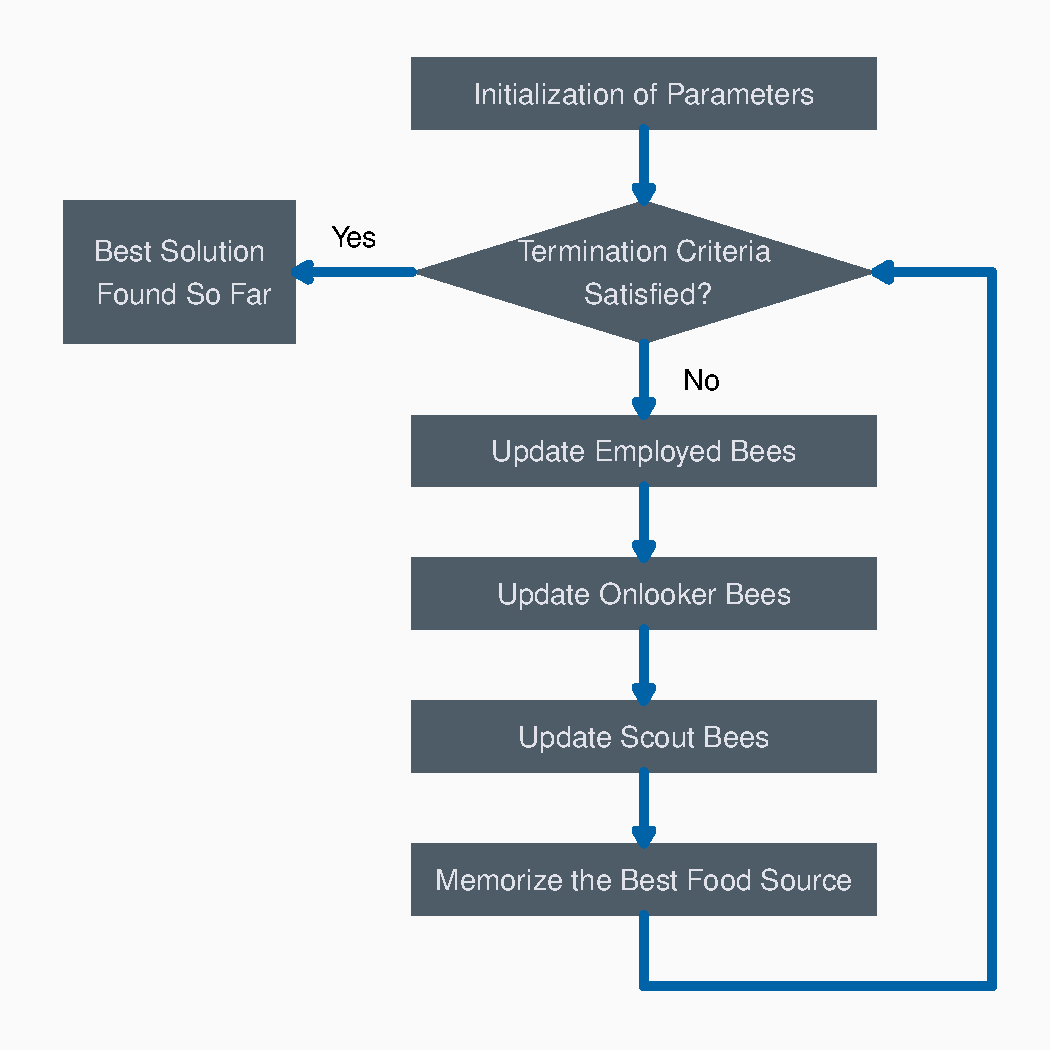
\includegraphics[width=0.63\linewidth]{pre1_files/figure-beamer/ABC-1} \caption{Phases of ABC. Source: Kumar, S. et al. (2014)}\label{fig:ABC}
\end{figure}

\end{frame}

\begin{frame}[fragile]{Initialization}
\protect\hypertarget{initialization}{}

\begin{Shaded}
\begin{Highlighting}[]
 \FloatTok{1.}\NormalTok{ Data}
 \FloatTok{2.}\NormalTok{ Generate the initial solution}
 \FloatTok{3.}\NormalTok{ Evaluate the }\KeywordTok{nectar}\NormalTok{ (fitness)}
\end{Highlighting}
\end{Shaded}

Parameters:

\begin{itemize}
\tightlist
\item
  The number of initial food sources \(SN=20\)
\end{itemize}

Simulation:

\begin{itemize}
\tightlist
\item
  Initial solution input\\
\item
  Initial food sources
\end{itemize}

\end{frame}

\begin{frame}[fragile]{Employed bees}
\protect\hypertarget{employed-bees}{}

\begin{Shaded}
\begin{Highlighting}[]
 \FloatTok{4.} \KeywordTok{While}\NormalTok{ (Condition not met)\{}
 \FloatTok{5.}\NormalTok{ For each employed bee\{}
\NormalTok{     Produce new solution }
\NormalTok{     Greedy selection \}}
\end{Highlighting}
\end{Shaded}

\begin{block}{Finding neighbour}

\[\nu_{ij} = z_{ij} + \phi_{ij}(z_{ij}-z_{kj})\]

\end{block}

\end{frame}

\begin{frame}[fragile]{Employed bees}
\protect\hypertarget{employed-bees-1}{}

\begin{Shaded}
\begin{Highlighting}[]
 \FloatTok{4.} \KeywordTok{While}\NormalTok{ (Condition not met)\{}
 \FloatTok{5.}\NormalTok{ For each employed bee\{}
\NormalTok{     Produce new solution }
\NormalTok{     Greedy selection \}}
\end{Highlighting}
\end{Shaded}

\begin{block}{Calculate fitness}

\[fit_i = \frac{1}{1+f_i}\]

\end{block}

\end{frame}

\begin{frame}[fragile]{Onlooker bees}
\protect\hypertarget{onlooker-bees}{}

\begin{Shaded}
\begin{Highlighting}[]
 \FloatTok{6.}\NormalTok{ Calculate the probabilities of solution}
 \FloatTok{7.}\NormalTok{ For each onlooker bee\{  }
\NormalTok{     Select a solution using probabilities}
\NormalTok{     Produce new solution}
\NormalTok{     Greedy selection \}}
          
\end{Highlighting}
\end{Shaded}

\begin{block}{Calculate probabilities}

\[p_i = \frac{fit_i}{\sum^{SN}_{i=1} fit_i}\]

\end{block}

\end{frame}

\begin{frame}[fragile]{Scout bees}
\protect\hypertarget{scout-bees}{}

\begin{Shaded}
\begin{Highlighting}[]
 \FloatTok{8.}\NormalTok{ Abandon non}\OperatorTok{-}\NormalTok{improving solution }
 \FloatTok{9.}\NormalTok{ Replace it with new solution}
\end{Highlighting}
\end{Shaded}

Parameter:

\begin{itemize}
\tightlist
\item
  The limit: 40
\end{itemize}

\pause

\begin{block}{Finding new solution}

\[z_i^j = z_{min}^j + \delta_i^j(z_{max}^j-z_{min}^j)\]

\end{block}

\end{frame}

\begin{frame}[fragile]{Stopping criteria}
\protect\hypertarget{stopping-criteria}{}

\begin{Shaded}
\begin{Highlighting}[]
\FloatTok{10.}\NormalTok{ Record the best solution }\ErrorTok{\}}
\FloatTok{11.}\NormalTok{ End}
\end{Highlighting}
\end{Shaded}

Parameters:

\begin{itemize}
\tightlist
\item
  Maximum number of iterations: 700
\item
  Maximum number of unimproved global minimum: 200
\end{itemize}

\end{frame}

\begin{frame}{Intensification vs Diversification}
\protect\hypertarget{intensification-vs-diversification}{}

\begin{block}{Local search}

Create new solution from neighbours

\begin{itemize}
\tightlist
\item
  The employed bee
\item
  The onlooker bee (with tendency)
\end{itemize}

\pause

\end{block}

\begin{block}{Global search}

Replace current solution using new solution found from solution space

\begin{itemize}
\tightlist
\item
  Abandon scheme
\item
  The scout bee
\end{itemize}

\end{block}

\end{frame}

\hypertarget{comparison}{%
\section{Comparison}\label{comparison}}

\begin{frame}{Escaping local optima}
\protect\hypertarget{escaping-local-optima}{}

Simulated annealing:

\begin{itemize}
\tightlist
\item
  Being able to accept worse solution based on temperature
\end{itemize}

\pause

ABC:

\begin{itemize}
\tightlist
\item
  Abandon solution that does not improve for many iterations (combined
  with global search)
\end{itemize}

\end{frame}

\begin{frame}{Reproduction}
\protect\hypertarget{reproduction}{}

\begin{columns}
\begin{column}{0.48\textwidth}

Genetic Algorithm:
\begin{itemize}
\item Selection
\item Crossover
\item Mutation
\item Evaluation
\item Update
\end{itemize}
\end{column}
\begin{column}{0.48\textwidth}

\pause

Each bee in ABC:
\begin{itemize}
\item Finding neighbour
\item Creating new solution
\item Calculating fitness
\item Greedy selection
\end{itemize}

\end{column}
\end{columns}

\end{frame}

\hypertarget{clustering}{%
\section{Clustering}\label{clustering}}

\begin{frame}{Adjustment}
\protect\hypertarget{adjustment}{}

\begin{block}{Solution representation:}

\(k\times D\) matrix \pause  \(\ \ \Rightarrow\) vector

\pause

\end{block}

\begin{block}{Standardization}

\(z^*_{ij} = \frac{z_{ij}}{\max_{}|z_{ij}|}\)

\pause

\end{block}

\begin{block}{Initialize different foods sources}

\begin{itemize}
\tightlist
\item
  Evenly assigned across the solution space \(\times\)
\item
  Randomly sampled between bounds \(\times\) \pause
\item
  Sampled from the existing data points
\end{itemize}

\end{block}

\end{frame}

\begin{frame}{Constraint and Relaxation}
\protect\hypertarget{constraint-and-relaxation}{}

Minimum cluster size: \(\frac{n}{2k}\)

Too hard to find a solution so we:

\begin{itemize}
\tightlist
\item
  Simulate initial input solution up to 4000 times
\item
  Initialize food sources up to 2500 times
\item
  Globally search in the scout bee up to 2000 times
\end{itemize}

\pause

Minimum cluster size is relaxed to \(\frac{n}{10k}\) if the algorithm
reaches the first two condition

\end{frame}

\begin{frame}{Result 1}
\protect\hypertarget{result-1}{}

\begin{center}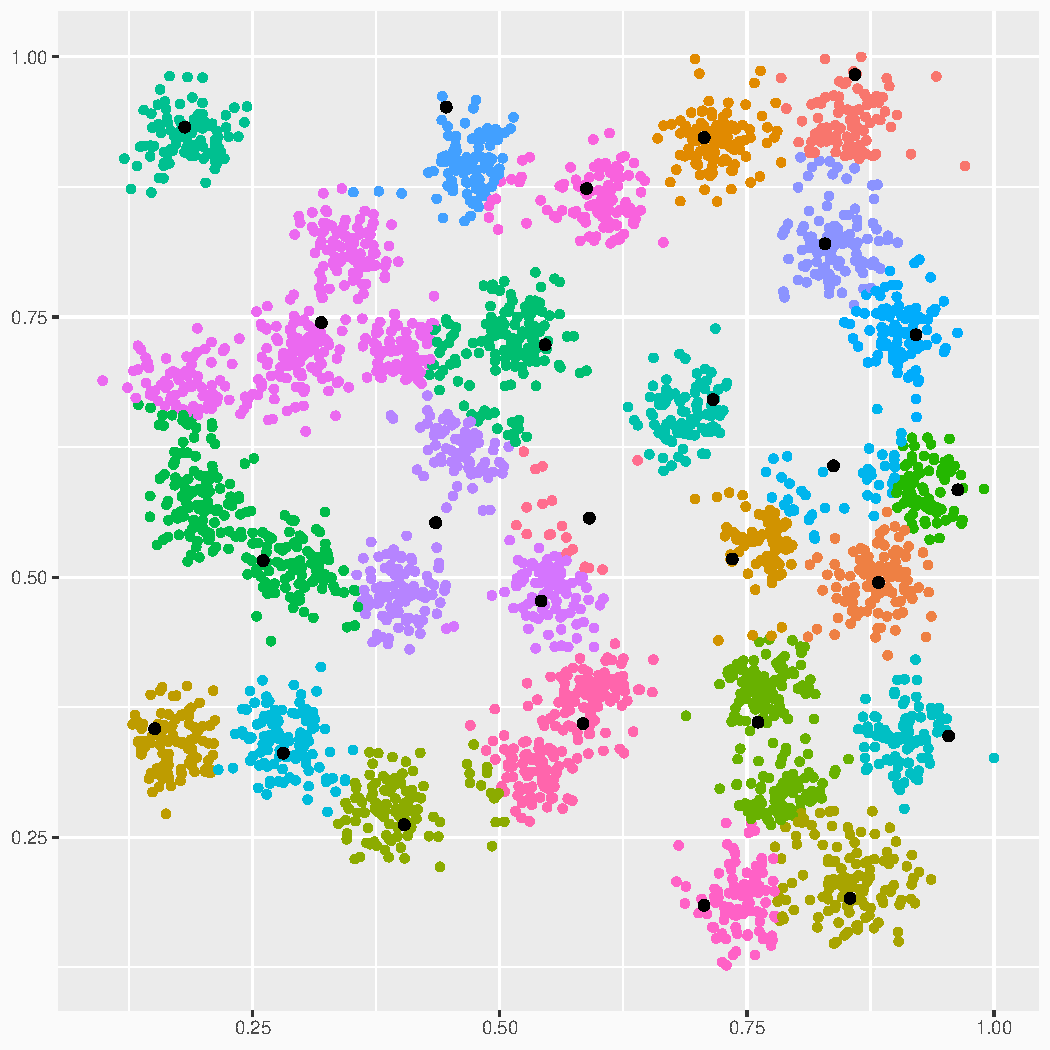
\includegraphics[width=0.7\linewidth]{pre1_files/figure-beamer/unnamed-chunk-1-1} \end{center}

\end{frame}

\begin{frame}{Result 2}
\protect\hypertarget{result-2}{}

\begin{center}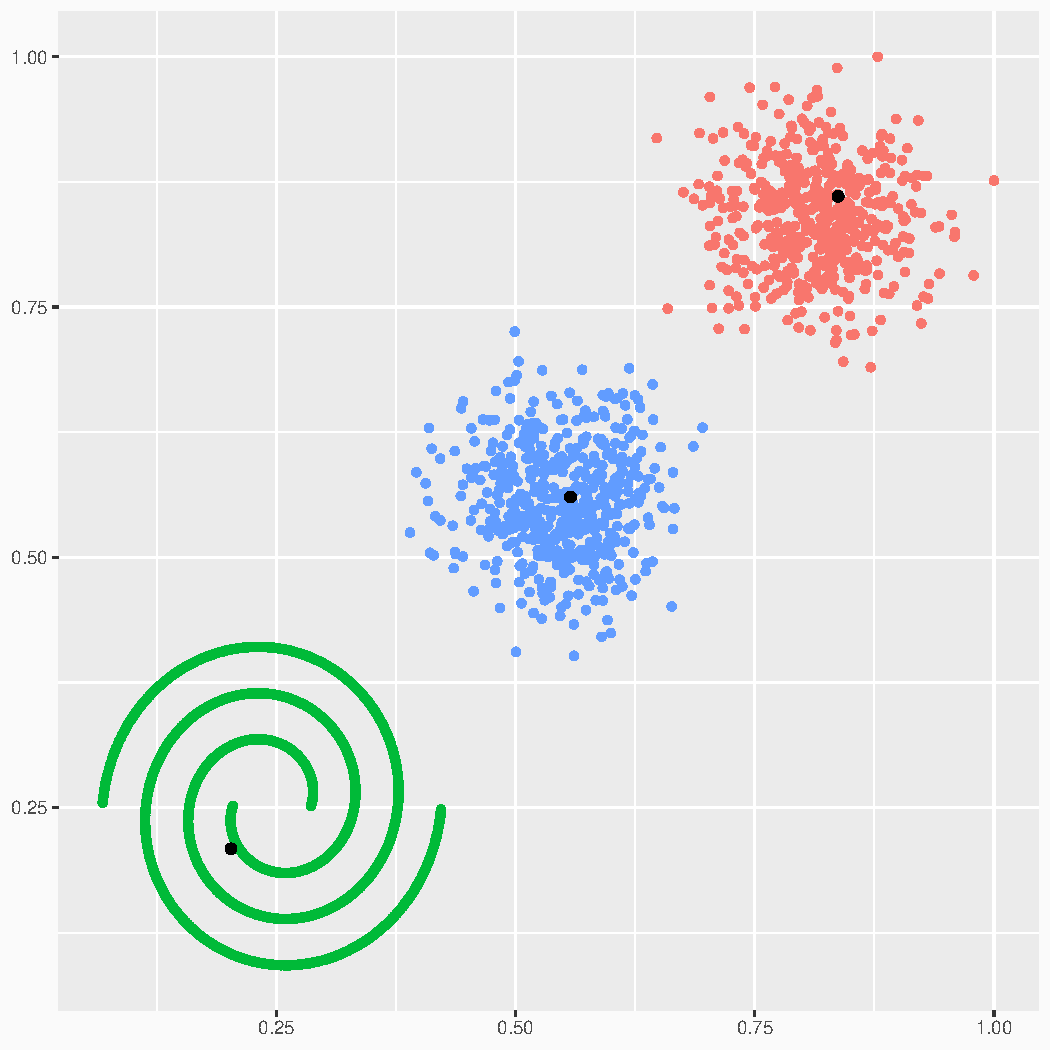
\includegraphics[width=0.7\linewidth]{pre1_files/figure-beamer/unnamed-chunk-2-1} \end{center}

\end{frame}

\begin{frame}[allowframebreaks]{References}
\protect\hypertarget{references}{}

Kumar, S., Sharma, V. K., \& Kumari, R. (2014). Randomized memetic
artificial bee colony algorithm. arXiv preprint arXiv:1408.0102.

\end{frame}




\end{document}
